\documentclass[11pt,sigconf]{iabart}
%\documentclass[10pt,sigconf,letterpaper]{acmart}
%\usepackage[vskip=1em,font=itshape,leftmargin=2em,rightmargin=2em]{quoting}
\usepackage[skip=4pt plus1pt]{parskip}
%\copyrightyear{2024}
%\acmYear{2024}
%\setcopyright{acmlicensed}\acmConference[IAB Network Management WS]{The IAB Next Era of Network Management Operations}{December 3, 2024}{}
%\acmBooktitle{The IAB next Era of Network Management Workshop}{December 3, 2024}{}

\begin{document}


\title{Evolving Challenges and Solutions in Network Management}

\author{Jaime Jiménez}
\email{jaime.jimenez@ericsson.com}
\orcid{0009-0008-2864-4269}
\affiliation{%
  \institution{Ericsson, ER}
  \city{Jorvas}
  \country{Finland}
}

\author{Scott Mansfield}
\email{scott.mansfield@ericsson.com}
\affiliation{%
  \institution{Ericsson, BNEW TS ST}
  \city{Jorvas}
  \country{Finland}
}

\author{Raquel Rodriguez A}
\email{raquel.a.rodriguez@ericsson.com}
\affiliation{%
  \institution{Ericsson, ETAC}
  \city{Jorvas}
  \country{Finland}
}

\author{Mikko Pesonen}
\email{mikko.pesonen@ericsson.com}
\affiliation{%
  \institution{Ericsson, ETAC}
  \city{Jorvas}
  \country{Finland}
}

\author{Vesa Torvinen}
\email{Vesa.Torvinen@ericsson.com}
\affiliation{%
  \institution{Ericsson, ETAC}
  \city{Jorvas}
  \country{Finland}
}


\begin{abstract}

This paper presents a comprehensive analysis of the evolving challenges and emerging solutions in network management. We explore scalability issues in network models and protocols, emphasizing the limitations of current implementations like YANG and the need for standardized, extendable models. Telemetry complexities are discussed, focusing on data quality, diversity, and lineage, and the necessity for efficient data streaming and standardized schemas. Security challenges are addressed in the context of diverse protocols and the transition towards zero-trust architectures, highlighting the importance of unified security mechanisms and continuous updates. We also examine the future of network management, including the integration of generative AI and agentic architectures that adhere to autonomic networking principles, as well as new standard interfaces like CoRECONF. Our findings underscore the imperative for scalable, secure, and interoperable solutions that can adapt to the dynamic demands of modern telecommunications networks.

\end{abstract}

\keywords{network management, scalability, telemetry, security, AI, zero-trust, interoperability}

\maketitle

\section{Introduction} \label{introduction}

The IAB workshop on the Next Era of Network Management Operations (NEMOPS) serves as a platform for discussion between network operators and protocol developers. This workshop is expected to guide the Internet Engineering Task Force (IETF) standards process. The workshop's primary objectives are to assess past achievements and delineate future requirements for network management operations.

In this paper, we introduce a comprehensive analysis of the current challenges and emerging solutions in network management from the point of view of an SDN controller product. The subsequent sections delve into various aspects of network management and operations. The \textbf{Overall Architecture} section \ref{overview} provides a detailed overview of the standard components within a network management controller, the Ericsson Transport Automation Controller (ETAC). The \textbf{Scalability} section \ref{scalability} examines the challenges of scaling network models and protocols, highlighting the need for standardized models. The \textbf{Telemetry} section \ref{telemetry} discusses the complexities of data transmission. The \textbf{Security} section \ref{security} raises some security challenges and explains the shift towards zero-trust architectures. Finally, the \textbf{Network Management Evolution} section \ref{insights} explores potential future trends, including the role of generative AI and new standard interfaces.

\subsection{ETAC overal Architecture} \label{overview}

Ericsson Transport Automation Controller (ETAC) ~\cite{ericsson-etac} is a cloud-native Transport Automation and SDN Controller that leverages artificial intelligence and machine learning to deliver advanced analytics and automation functionalities across microwave, IP, and optical fronthaul networks.

\begin{figure}[h]
  \centering
  \includegraphics[width=0.5\textwidth]{figs/arch.pdf}
  \caption{General Architecture}
  \label{fig:overall_architecture}
\end{figure}


The \textbf{Ericsson Network Manager (ENM)} is a centralized platform responsible for managing network and service discovery, as well as collecting performance metrics. ENM interfaces with network elements like microwave nodes, known as \textbf{MINI-LINK}, to gather critical performance management (PM) data using \textbf{SFTP} \cite{RFC4253}.

ENM also exposes network topology and service information to external systems through its Configuration Management Northbound Interface (CM NBI) over \textbf{HTTP/S} \cite{RFC7230}, enabling seamless integration with other platforms. This allows \textbf{Network Management Users} to monitor and control the network environment via a secure web-based interface.

On the other side of the ecosystem lies the \textbf{ETAC} platform \cite{ericsson-etac}, an AI-enhanced tool designed to provide deeper insights and advanced analytics. ETAC communicates with ENM to retrieve PM data via \textbf{SFTP} \cite{RFC4253}, ensuring it has the necessary information to optimize network performance. ETAC also interfaces with MINI-LINK directly, using \textbf{SNMP} \cite{RFC1157} to receive real-time microwave link parameters. These parameters help ETAC maintain a granular view of the network's operational status.

Furthermore, ETAC leverages \textbf{NETCONF/YANG} \cite{RFC6241, rfc6020} to configure and manage RDS (Radio Data System) and service parameters within MINI-LINK. This protocol enables precise, programmatic control over network devices, aligning with the industry's shift towards more automated and dynamic network configurations.

Finally, both platforms provide secure \textbf{HTTP/S} \cite{RFC7230} interfaces for their respective user bases—ENM for Network Management Users and ETAC for ETAC-specific users. 


\section{Scalability} \label{scalability}

% Challenges of scalability in network models/protocols/devices/systems
% Optical equipment that can have up to 10,000 interfaces. Current models like YANG are inadequate due to limitations such as file databases without indexing.
% There is a need for standardized network-level models that can be easily mapped to devices, facilitating scalability across various network architectures.
% The integration of legacy systems remains a significant challenge, with many network nodes still relying on SNMP, necessitating adaptable and scalable solutions.
% Stateful connections vs stateless
 

\textbf{YANG Schema Mount}

Scalability in YANG presents significant challenges, as highlighted by Boyd \cite{boyd2023scalable}. The concern is about the viability of the current implementation of YANG Schema Mount \cite{RFC8528} and the need to support a mechanism that is better suited for partitioning the data in the hierarchical data tree.

% This needs to be rewritten to human-level of understanding.
Even an enhanced solution for this issue will really only be solved by a better underlying modeling implementation including ACID/transactional, time-series, object-relational views with a query-language and the ability to add triggers or embedded code that becomes part of the solution. The complexity of YANG is intensifying, largely driven by its hierarchical architecture.

\textbf{Efficient Data Streaming for Analytics}

The efficient and scalable transfer of analytics data from its source to post-processing systems remains a significant challenge. Legacy network elements predominantly rely on periodic data harvesting, which imposes unnecessary load on the network elements and delays data accessibility. To address this, data sources should implement active streaming of data to post-processing systems immediately upon production. This approach ensures that post-processing systems and closed-loop automation have access to data in near real-time.


\section{Telemetry} \label{telemetry}

% The challenges of using UDP for telemetry.
% Need for fine-grained control over data transmission.
% Observability in retrieving records without overwhelming the DCN(?)
% Handling of mmulti-protocol data and reporting mechanisms. Traps, YANG push, coap observe...
% YANG to CBOR dictionary for compression and the implications of frequent notifications.
% Signaling using lightweight protocols


% Concise Binary Object Representation (CBOR) compresses YANG modules for transmission via the Constrained Application Protocol (CoAP) \cite{RFC9254, rfc7252}. This is advantageous for devices in Low-Power and Lossy Networks (LLNs), which have limited power and memory. CBOR optimizes data transmission and enhances network efficiency in such environments.


\textbf{Quality of data} 

Legacy network elements generate data that is not optimized for modern IT-style post-processing analytics systems. This data requires embedded metadata within its schema to support long-term storage and external post-processing, detailing the "what, where, when, and by whom," and identifying the precise source, such as a container, pod, application, node, or CaaS-cluster.

Currently, the lack of alignment in analytics data schemas and metadata complicates and increases the cost of post-processing and analytics. Simple discrepancies, like varying timestamp formats, can cause significant issues. Ideally, standardized, extendable schemas and encodings for different analytics data types would simplify data processing across diverse vendor systems.

Reliability of telemetry data may be less critical when used for visualization purposes and manual check-ups, however, it becomes crucial once telemetry is used as input for AI training and assisted network configuration

\textbf{Diversity of data} 

Currently, analytic data is accessed through various APIs and follows diverse patterns (e.g., file harvesting, SNMP for FM data streaming, state notifications via NETCONF/RESTCONF, etc). This diversity complicates data collection and ingestion processes. There is a pressing need for an efficient, scalable, and universal transfer system to stream analytics data from its source to post-processing systems. This system must be optimized for bandwidth and CPU efficiency, ensure security, and be applicable to all types of analytics data streams, including metrics, events (e.g., alarms and notifications), logs, and state data.

\textbf{Lineage of data}

It is essential to establish the lineage and integrity of any record used for purposes beyond visualization. Utilizing data with uncertain integrity can introduce new attack vectors, such as enabling adversaries to exploit closed-loop automation by manipulating the input data. It is important to note that analytics data may flow directly from the source to the post-processing system; however, there are instances where data may traverse cloud provider PaaS functions. Therefore, a mechanism to ensure data integrity across multiple domains is necessary.

\textbf{State-Data Handling}

% This needs to be rewritten more clearly
In passive data sources where analytics data is just exposed (as opposite to streamed) the data has to be actively harvested by external entities, thus there must be APIs or interfaces for collection of such data. In systems where data is streamed, the data sources (often involved in critical functions such as traffic handling) do not need to expose interfaces for harvesting analytics data, which makes the attack surface smaller and system more secure in general.

Modern network elements have a lot of state-data which can not be efficiently leveraged through config model notifications. There are components and elements in the applications/data sources, which one does not to expose in a model, but still the analytics data about the state of such components should be available for post-processing systems. For example, one ideally would like to keep the model of cloud service realization agnostic, and use the same model for the cloud service, whether the application-instances of those services run in virtual machines or in container. Having to model compute resources in order to convey the state data would make it very tricky to separate realization and model from each other, and keep the model backwards compatible as the application realizations evolve and technologies change.

\section{Query Range} \label{queryrange} 

% Importance of protocol-agnostic network modeling, which allows for a broad query range.
% Database storage and retrieval. Time-series storage. 
% The meeting discussed the differences between UML-defined models and those used in YANG, focusing on how these models can operate in a protocol-neutral manner.

TBD!

\section{Security challenges} \label{security}

Security configuration in network management is complex due to the absence of a unified infrastructure. This complexity arises from the need to support multiple security protocols across diverse devices and vendors. Key points include:

\begin{itemize}
    \item \textbf{Diverse Protocols:} Network management applications must accommodate various security protocols, such as TLS, SSH, and username/password mechanisms.
    \item \textbf{TLS Potential:} TLS, especially with client-server certificates, is a strong candidate for unified security but lacks universal support across all network management protocols and devices. %IS THIS TRUE???
    \item \textbf{SSH Limitations:} there is no security infrastructure available that would distribute and help verifying the SSH public keys and facilitate flexible re-keying.The security configuration of SSH itself remains to be manual.
    \item \textbf{Username/Password Usage:} Widely used for basic access and protocols like SNMPv3. Mechanisms for centralized authentication exists but cannot completely replace the need for local authentication because centralized mechanisms may not be always available. Manual security configuration leads easily to poor security practises as key renewals, password upgrades are easily neglected simply because it is error prone and expensive.

\end{itemize}
 

\textbf{Standardization process}

The transition from standards to widespread network deployment is often very slow, particularly when new standards are to replace existing components. While implementing a new mechanism on a single device can be swift, updating all network devices is time-consuming. Management applications typically require market adoption or commitment to the new mechanism before implementation is deemed worthwhile. For this reason, phasing out legacy security mechanisms is challenging.
 
\textbf{Zero-Trust Architecture}

Ericsson develops products that are configured to use secure protocols and configurations by default. But we still see in legacy networks that sometimes the transport network is assumed to be secured, trusted, so that a lower degree of security is sometimes accepted. This may work in some networks but the trend is definitely towards zero-trust. 

Regulators and local legislation is also setting new requirements for critical infrastructure, such as telecom networks. The interest is not only on the security capabilities required from the network devices but also development processes, documentation, FOSS usage, security assurance and various aspects of the way how networks are deployed and managed.

One unfortunate reality is that some network devices in life networks are actually very old. If the network operates correctly, any upgrade or change to it may start looking like a risk. This may lead to neglection of software and security upgrades. This could work in the walled-garden paradigm but definitely not anymore in zero-trust. Continuous deployments and upgrades are the only path to truly secure networks. And all this would need to be automated in secure way, covering the software upgrades, re-configurations and testing.

 
\section{Network Management Evolution} \label{insights}


% Maybe GenAI and Intents?
% Other db/api query languages? GraphQL
% Other, new standard interfaces?
% More closed-loop Automation?
% Workflow Programmability and Network APIs (Ericsson message)?


\textbf{AI Agents}

Zero-shot LLMs are are already used to make operator insights more accessible, to streamline incident management or to generate task-specific code from natural language queries. As the industry progresses in the GenAI path, agentic architectures will be integrated into network AI systems, adhering to the autonomic networking principles specified in RFC7575.

\begin{quote}
"The fundamental goal is self-management, including self-configuration, self-optimization, self-healing, and self-protection." \cite{RFC7575}
\end{quote}

Agentic systems are characterized by AI agents that are capable of decomposing user intents into executable individual steps and can interact autonomously with other systems through well-known interfaces (e.g., Network and Management APIs). Agents can further federate and specialize in multi-agent systems, which improve on challenges such as hallucinations, specialization, and scalability. The interest in multi-agent systems was reflected during the past IETF 121 side meeting, as detailed in the ai4network agenda \cite{ai4network-agenda}. 

\begin{figure}[h]
  \centering
  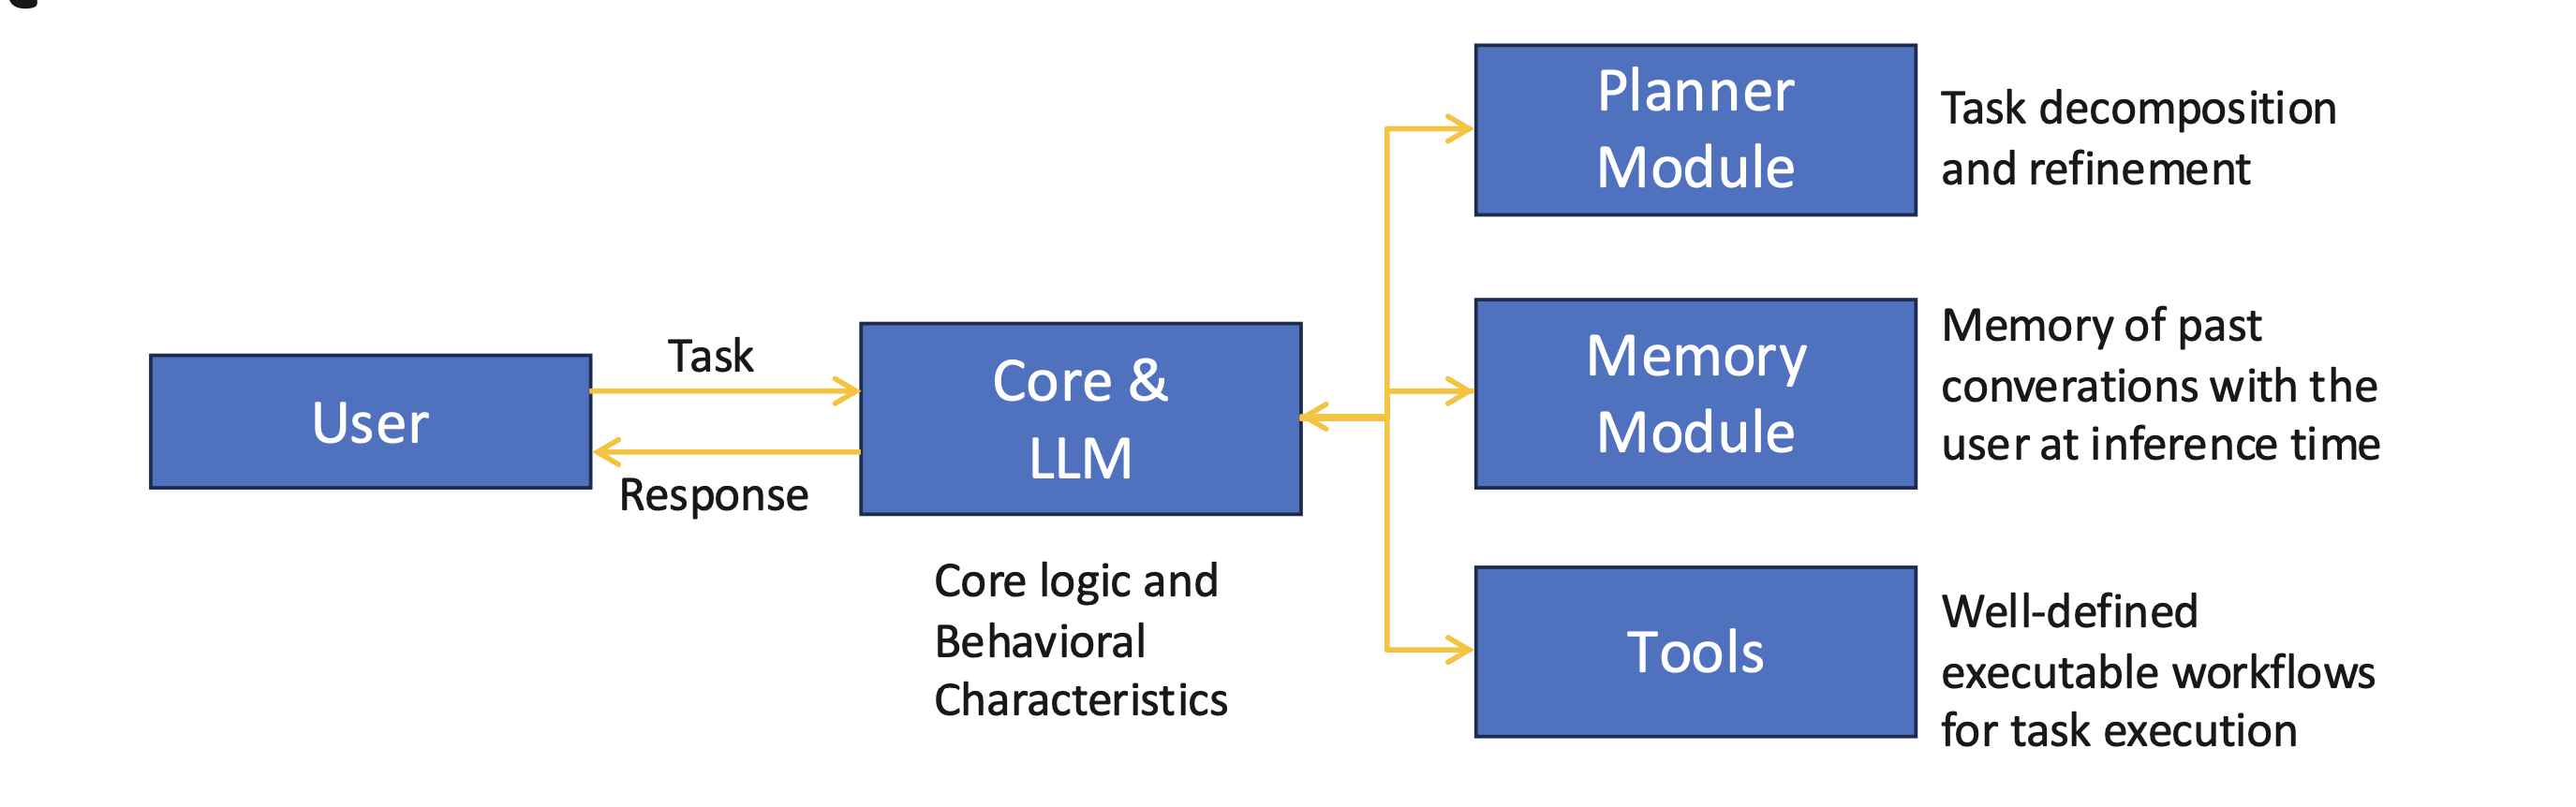
\includegraphics[width=0.5\textwidth]{figs/agent.png}
  \caption{Agentic System Architecture}
  \label{fig:agent_architecture}
\end{figure}

Agents are particularly useful in the telecommunications sector, where the complexity of specifications and codebases demands innovative solutions. Moreover, the current trend in 5G Networks is marked by a shift towards exposing network functionalities through APIs. This trend facilitates the integration of agentic systems that can dynamically interact with these APIs.

\textbf{CoRECONF}

The -CONF ecosystem comprises the following components:
\begin{itemize}
  \item \textbf{NETCONF} \cite{RFC6241}: Serializing YANG over a stateful TCP connection.    
  \item \textbf{RESTCONF} \cite{RFC8040}: Serializing YANG over stateless HTTP.
  \item \textbf{CoRECONF} \cite{draft-ietf-core-comi}: Serializing YANG modules in a CBOR \cite{RFC9254} map over stateless CoAP.
\end{itemize}

CoRECONF, in particular,is utilized by constrained devices in Low-Power and Lossy Networks, which are typically composed of numerous embedded devices with limited power and memory. Although primarily used for IoT, CoAP has also been specified for the signaling of DDoS-related telemetry \cite{RFC9132} and \cite{RFC9362}, as outlined in the now-concluded DOTS Working Group. 

This suggests potential applications for retrofitting CoAP on telemetry or management-type signaling within the network management domain. Specially in UDP-oriented evinronments as CoAP comes with an additional reliability mechanism and in environments where compression and smaller payloads are welcomed. 

\section{Conclusions} \label{conclusions}

This paper has explored the evolving landscape of network management, highlighting the challenges and solutions in scalability, telemetry, and security. The integration of advanced technologies such as AI and machine learning within platforms like the Ericsson Transport Automation Controller (ETAC) demonstrates the potential for enhanced analytics and automation in network operations. However, the complexity of legacy systems and the diversity of data sources present significant hurdles that require innovative approaches, such as standardized schemas and efficient data streaming mechanisms.

The transition towards zero-trust architectures and the adoption of generative AI indicate a shift towards more secure and autonomous network management systems. These advancements necessitate a collaborative effort between industry stakeholders and standardization bodies to ensure seamless integration and widespread adoption. As the network management domain continues to evolve, the focus must remain on developing scalable, secure, and interoperable solutions that can adapt to the dynamic demands of modern telecommunications networks.

\section{Acknowledgments}

We would like to thank Ericsson for their support of this work. Special thanks to ...


\bibliographystyle{ACM-Reference-Format}
\bibliography{paper}

\end{document}
\endinput


% NOTES

% ------------------------------------------------------------------------
% WS CALL
% ------------------------------------------------------------------------
% Common protocol themes: YANG, YANG-Push, NMDA, NETCONF, RESTCONF, CORECONF, SZTP, Call-Home, YANG-Library

% Current IETF network management topics:
% NETCONF (NETwork CONFiguration) WG
% NETCONF-next, RESTCONF-next, configuration of clients and servers, list pagination, transaction correlation, YANG-push transports (Protocols and YANG models)

% NETMOD (NETwork MODelling) WG
% YANG-next, YANG versioning, system configuration, data immutability (Language and YANG models)
% NMOP (Network Management Operations) WG
% YANG-push integration with Apache Kafka & time series databases, anomaly detection and incident management, digital map modelling

% Network Inventory (IVY) WG
% Hardware & software components, physical location, etc. correlating with existing IETF models (topolopy, service attachment points)

% Discussion topics will include, but are not limited to:
% 	•	Tooling, open source, experimentation, proof of concept, multi-vendor interoperability test (e.g., EANTC), and system integration
% 	•	Data consistency to support richer observability (Data & Knowledge)
% 	•	Integration issues with the business layer
% 	•	Automation, orchestration, and autonomy
% Goal is to Explore new requirements for future network management operations in a collaborative manner with the industry, network operators, and protocol engineers

% Check examples in slides: https://ripe89.ripe.net/wp-content/uploads/presentations/47-RIPE89_Next_Era_of_Network_Management_Operations_Benoit_Claise.pptx

% ------------------------------------------------------------------------

% ------------------------------------------------------------------------
% MEETING Nov4
% ------------------------------------------------------------------------

% NEMOPS Paper
% Signaling using lightweight protocols
% IVY topic
% Mention a bit the liaison, industry recognize center of competence. Connection between IETF, … ITUT
% - Scalability
% - Query range
% - Telemetry

% ETAC Telemetry: UDP examples of struggles and issues, fine-grained granular control of what gets push. High level describe what we do currently.  The reality of when developing these products you have to live in the legacy and the new world. Adaptors, many items in nodes are still SNMP, the reality is that u have to deal with a lot of legacy. Network modeling can be agnostic of the protocol used, network modeling can be abstracted to the method u use to the network elements.

% ITUT difference between the models we define in UML and the ones we used in YANG, how things work in a protocol neutral way (MIB, YANG…) the industry was not ready for it back then. If you have a practical example …

% Internally we have an adaptation layer towards the managed devices. 
% Scott: standardize that?
% When defining those network level models there should be a mapping between those network level models and device, so that they can be mapped easily. Scalability: optical equipment with 10k interfaces YANG does every poorly. File database with no indexing. Scott has a press about that. Redo the modeling of the bridge. 
% Compression: YANG to CBOR, something to think, if net elements notifications every 10s the smaller the better, fits also with the telemetry topic.

% Telemetry: Observability to get back records. Do not want to kill the DCN. When you get stuff back, you have a value and put it somewhere, you can do traps, yang push, if you put it in a database, I don't know if we have standard that maps it to that. Tool somewhere that maps. RESTCONF: Got stop time-series databases and relational databases. 
% GraphQL